\documentclass[twocolumn]{article}

% To render inline code
\usepackage{listings}
\lstset{basicstyle=\ttfamily}

% For the bibliography 
\usepackage[round]{natbib}
\bibliographystyle{plainnat}

% Render the equations
\usepackage{amsmath}

\usepackage{graphicx}

\title{How and why to quantify pairwise pleiotropy}

\begin{document}
	
	\author{Thomas James Ellis}

%----------------------------------------------------------------------------------------
%	ARTICLE CONTENTS
%----------------------------------------------------------------------------------------
\twocolumn[
\begin{@twocolumnfalse}
	\maketitle
	\begin{abstract}
		Abstract text.
	\end{abstract}
\end{@twocolumnfalse}
]

\section{Introduction}

Pleiotropy is when a single locus affects two or more traits.
It is of particular interest in evolution because it can either facilititate evolutionary change when multiple traits are selected in parallel, or constrain it when traits trade-off with one another.
Pleiotropy is thought to play and important role in trade-offs between life history traits such as longevity and reproduction, adaptation to contrasting environments, and the degree to which phenotypic complexity constrains evolution \citep{Williams1966a, williams1957pleiotropy, Stearns1992,Kawecki2004, wagner2008pleiotropic}.
One fruitful line of research has been to characterise pleiotropy by measuring its effects on correlations between phenotypes \citep{Stearns1992}.
With the more recent advent of molecular and statistical techniques to identify the genetic basis of traits we have begun to address the challenges involved in understanding the pleiotropic mechanisms acting at individual loci \citep{mitchell2007evolutionary, wagner2011pleiotropic, Wadgymar2017}.

Three mechanisms are typically invoked to describe pleiotropic effects of alleles on pairs of traits \citep{Kawecki2004, mitchell2007evolutionary, Hall2010}.
First, negative (or antagonistic) pleiotropy occurs when an allele is associated with an increase in the trait in one trait, but a decrease in the second trait.
Second, positive pleiotropy occurs when an allele is associated with an increase in both traits, or a decrease in both traits.
A third "non-pleiotropic" case occurs when an allele is associated with a change in one trait, but no change in the second.
When the traits in question are fitness in two environments, the latter case is often referred to as 'conditional neutrality' \citep{mee2019unpacking}.
These mechanisms have obvious parallels to positive, negative and zero genetic correlations between overall phenotypes.
Moreover, the more loci that show negative pleiotropy, the more negative the genetic correlation will be, and hence the stronger any trade-off, and vice versa.
The frequency of each pleiotropic mechanism is therefore central to determining the relationships between traits, and how they constrain one another.

To understand trade-offs it is essential to be able to measure them.
For example, relationships between traits can be measured as genetic correlations \citep{Falconer1996, Stearns1992}.
The resulting correlation coefficient provides an quantitative, intuitive measure of the direction and magnitude of the relationship, which can be easily tested against a null hypothesis.
However, this relies on having a sample of many genetically diverse individuals on which to measure phenotypes.
To investigate the pleiotropic effects of individual loci we can only measure the effect of one allele against the other on each trait in question.
A typical approach is to perform a statistical test on the effect on each trait, and classify loci affecting neither, one or both traits.
However, as we outline in detail below, this classification process ignores the fundamentally continuous nature of the problem and leads to a statistical bias that systematically underestimates the amount of pleiotropy in the system \citep{hill2012pleiotropic}.
Just as correlations measure not just the direction, but also the strength of a relationship between traits, what we need is a framework to quantify the direction and strength pleiotropic mechanisms.

In the rest of this paper we identify and review three key reasons why current approaches to measuring pleiotropy are flawed, and use these to motivate a quantitative framework for measuring trade-offs for individual genotypes.
We focus on pleiotropic effects of alleles at individual loci, but note that this framework is equally applicable to pairs of multilocus genotypes measured in two contexts, such as a local and a non-local ecotype.
We then apply this framework to empirical datasets in \textit{Arabidopsis thaliana} investigating environmental and physiological trade-offs in fitness traits.
An R package \lstinline|psiotropy| is provided to apply the method described, available from URL.

\section{Null-hypothesis tests bias conclusions}

% \begin{figure}
% 	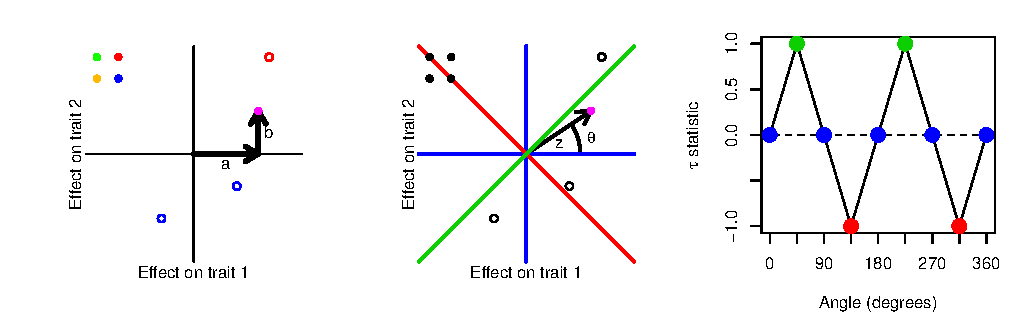
\includegraphics[width=\linewidth]{fig1.eps}
% 	\caption{A boat.}
% 	\label{fig:theory}
%   \end{figure}

\begin{figure*}
    \centering
    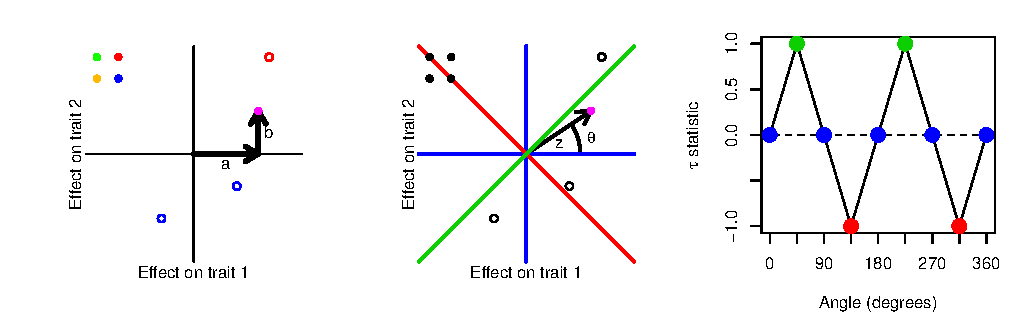
\includegraphics[width=\textwidth]{fig1.eps}

    \caption{Two ways to measure pleiotropy. Each point shows the effect of a hypothetical locus on traits 1 and 2. Colours indicate pleiotropic mechanism: red, green and blue points indicate loci showing negative, positive and zero pleiotropy; black points show no significant association with either trait. (A) Null-hypothesis tests of allelic effects on each trait. A reference allele at each locus has effects \textit{a} and \textit{b} on traits 1 and 2 respectively, and the statistical tests are performed along the x- and y-axes. The grey bars indicate the boundary of statistical significance. Each locus is categorised as affecting zero, one or both traits based on which side of the bars they are located. (B) The same loci, but represented as vectors with angles ($\theta$) and lengths (of magnitude \textit{z}) from the origin. (C) Function $\psi$ relates angles to pleiotropic mechanisms. Three special cases when $\psi$ is -1, 0 or 1 correspond to antagonistic pleiotropy (red), zero pleiotropy (blue) and positive pleiotropy (green) respectively. Values between these points measure everything in between.}
    \label{fig:theory} % Label for end{figure*}
\end{figure*}

We consider a biallelic locus associated with two traits typical of many studies.
The reference allele at this locus is associated with a change in trait 1 of size $a$ in trait 2 of size $b$ (Fig. \ref{fig:theory}A).
The most appropriate way to estimate $a$ and $b$ will depend on the study system, but it is essential that the distribution of effects on traits 1 and 2 be symmetrical around zero so that the choice of allele is arbitrary, and on the same scale for both traits so they can be compared.
For quantitative phenotypes this can be acheived by standardising values by their mean and standard deviation \citep{schielzeth2010simple}.
For measures of fitness and its components, one can use the log relative fitness of two alleles.

The next step typically involves some kind of statistical test for the null hypotheses that $a$ or $b$ are zero.
A common approach is to perform two univariate tests for each trait separately, often accompanied by a discussion of the relative direction of the effect on each trait (e.g. \citet{wagner2008pleiotropic, Hall2010, anderson2011life, agren_genetic_2013, ellis2021life}).
Loci that are significantly associated with both loci are classified as positively or negatively pleiotropic (the red points in Fig. \ref{fig:theory}A), those associated with only one trait as showing zero pleiotropy (blue points in Fig. \ref{fig:theory}A), and those affecting neither trait are ignored (black points in Fig. \ref{fig:theory}A).
We note that other testing variants are available, such as tests for whether a locus affects both or either trait (e.g. \cite{korte2012mixed}; see \cite{porter2017multivariate} for a review and comparison).
Nevertheless, the goal is the same: to classify each locus as affecting one, both, or neither trait via null hypothesis testing.

There are three shortcomings with this approach.
First, by classifying effects based on significance thresholds we ignore useful quantitative information about pleiotropic mechanisms.
For example, if we classify the loci in Fig.~\ref{fig:theory}A based on how many traits they each affect we would infer that the red loci shows negative pleiotropy, the blue loci no pleiotropy, and we would ignore the black loci as non-significant.
In fact it is clear that loci are often much closer to points of other pleiotropic mechanisms than they are to loci of the same colour.
As an example, look at the solid points in Fig.~\ref{fig:theory}A; the effects of these loci are all broadly associated with a decrease in trait 2 and an increase in trait 2.
However, they happen to fall on either side of significance threshold, and are classified as having distinct pleiotropic mechanisms.
By classifying pleiotropic mechanisms into discrete categories based on statistical significance at individual traits we ignore quantitative information about the strength and mechanism of pleiotropy.

Second, to identify a pleitropic effect on two or more traits this way requires that we identify two or more statistically significant null-hypothesis tests.
However, it will always be a priori more difficult to find two significant associations than one \citep{wagner2011pleiotropic, hill2012pleiotropic}.
Using a standard significance threshold of p=0.05, the a priori expectation of identifying an association with a single trait is 0.05.
The expectation of finding two significant associations is $p^2=0.00625$, or twenty-fold less likely.
Higher-order pleiotropic interactions become exponentially more difficult to find.
For a visual intuitiion for this, observe that loci classified as pleiotropic in Fig.~\ref{fig:theory}A must fall into the corners of the diagram.
These are the very regions that are furthest from the centre, meaning that effects have to especially strong to be classified as pleiotropic.
This effects leads to a statistical bias that systematically underestimates the amount of pleiotropy in the system.

Third, use of significance thresholds biases the kinds of effect sizes deemed to be important.
It is well known that unless sample sizes are large, conditioning on significant associations tends to overestimate effect sizes \citep{beavis1998qtl, xu2003theoretical}.
This also means we filter out any loci deemed to be 'non-significant'.
The extent to which these matter will depend on the biological question, but quantitative traits that are generally expected to have a substantial contribution from loci with weak to moderate effects, but which can have a substantial contribution to genetic variance in aggregate \cite{Fisher1930}.
Rather than remove them, a stronger approach would be to quantify how much weak effects contribute to overall trade-offs.

In summary, by relying on null-hypothesis testing to infer mechanisms of pleiotropy we (1) discretise what is a continuous phenomenon, (2) underestimate the amount of pleiotropy, and (3) ignore the contribution of weak effects. To alleviate this, we would like a method that (1) quantifies rather than classifies pleiotropic mechanism, (2) focusses on effect sizes and their uncertainty, and (3) uses as much of the data as possible.

\section{Quantifying trade-offs}

\subsection{Effects as angles and magnitudes}

We propose a simple approach to address the goals identified in the previous section.
Rather than define pleiotropic effects along the axes of traits 1 and 2 (Fig. \ref{fig:theory}) we instead describe effects as angles and vector lengths.
Any pair of values for $a$ and $b$ can be described via angle $\theta$ and magnitude $z = \sqrt{a^2+b^2}$ (Fig. \ref{fig:theory}B).
$\theta$ is measured (arbitrarily) from the axis pointing right, and contains information about the mechanism of pleiotropy.
When $\theta$ points along the axes in red, blue and green in Fig. \ref{fig:theory}B these correspond to loci showing negative, zero, and positive pleiotropy respectively.
Note that, as mentioned above, this relies on $a$ and $b$ centered around zero and on the same scale.

$\theta$ can be turned into a more useful statistic by taking function $\psi$ (Fig. \ref{fig:theory}C)
This function is cyclical and hence must be defined piecewise:

\begin{equation}
\psi=
\begin{cases}
     k\theta, & \text{if}\   0^\circ \geq \theta <  45^\circ \\
   2-k\theta, & \text{if}\  45^\circ \geq \theta < 135^\circ \\
  -2+k\theta, & \text{if}\ 135^\circ \geq \theta < 225^\circ \\
   2+k\theta, & \text{if}\ 225^\circ \geq \theta < 315^\circ \\
  -2+k\theta, & \text{if}\ 315^\circ \geq \theta < 360^\circ
\end{cases}
\end{equation}

where $k=\frac{1}{45}$.
This resembles a linearised sine wave, and is likely to be clearer as a figure (Fig. \ref{fig:theory}C) than an equation.
Values of $\psi$ of -1, 0, and 1 correspond to the special cases of symmetrical negative, zero and positive pleiotropy (red, blue and green in Fig. \ref{fig:theory}B and C).
However, since $\psi$ is quantitative, all intermediate values between these cases are possible.
There is a close analogy here with traditional correlation coefficients, where values from -1, 1 reflect a continuum from negative to positive correlations.
In this way, $\psi$ reflects an intuitive quantitative measure of the pleiotropic mechanism.

The overall length of the vector $z$ reflects the overall magnitude of the effect.
Just as larger values of $a$ and $b$ reflect stronger effects on each trait, values of $z$ which are further from the origin reflect a stronger effect overall.
A key difference between these numbers is that $a$ and $b$ measure effects along specific axes, but $z$ but is agnostic about the direction of the effect.
This decouples estimation of the direction and magnitude of the effect.
This also means that estimates of uncertainty can be assessed on one axis only, negating the need to test multiple traits at once.

\subsection{Uncertainty in estimates}

In addition to point estimates of $\psi$ and $z$ one would typically wish to estimate the uncertainty of these statistics.
Two points are worth highlighting here.
First, if we were to compare vectors of different magnitudes of $z$, we would expect shorter vectors to have higher uncertainty in $\psi$, even if the standard errors of $a$ and $b$ remained constant (Fig \ref{fig:uncertainity}A).
As $z$ approaches zero, the overlap becomes complete, and there is no information about the $\psi$.
Fortunately, this is indpendent of the direction of $\theta$.
The stronger the allelic effects the more robust are estimates of pleiotropic mechanism.

Second, pleiotropic traits of interest are often correlated.
This in turn causes the sampling distributions of $a$ and $b$ to be correlated.
The direction of this correlation can have a major impact on uncertainity in $\psi$.
When the directions of $\psi$ and the correlation of sampling distributions are closely aligned, we expect less uncertainty in $\psi$.
When the directions are opposite, we expect greater uncertainty in $\psi$.
By extension, if we were to incorrectly assume the correlation were zero we would estimate the uncertainty in $\psi$ incorrectly.
As such, care must be taken that any resampling procedure accounts for the correlation in the sampling distribution of $a$ and $b$.

A simple way to estimate uncertainity in pleiotropy statistics is to generate a sample of estimates of $a$ and $b$ and calculate $\psi$ and $z$ on each pair of values.
It is then straightforward to calculate confidence intervals from the quantiles of those distributions.
This can easily be done by non-parametric bootstrapping, which when done correctly should preserve the covariance structure between $a$ and $b$ \citep{efron1982jackknife}.
Other approaches would be parametric bootstrapping or Bayesian regression, as long as care is taken to model the covariance.

% The closer $z$ is to zero, the more the distribution of $a$ and $b$ overlap zero, and the greater the uncertainty in $\psi$.
% Thus, the degree of overlap reflects a quantitative estimate of the robustness of estimates of $\psi$.
% To estimate this, we first project the sample of values for $a$ and $b$ onto the vector $\bar{a},\bar{b}$, and calculate the magnitude $z*$ of those projections.
% We then estimate $q$ as twice the proportion of projected points which are on the same side of the origin as $\bar{a},\bar{b}$.
% When no points overlap, this number is 1; as $z$ approches zero, $q$ approaches 0.

% How to claculate zstar
% get a q

% Sometimes you might not be able to do that.
% Here's a formula to get a SD on z.

% \subsection{\verbatim{sintillate} package}

% \section{Application to data}

% \subsection{Pleiotropy in local adaptation}

% Selection on parental phenotypes

% Selection across markers

% Somehow relate (mean?) tau to genetic correlation? 

% %------------------------------------------------

\section{Discussion}


There is a close correspondence between $\psi$ 
just as genetic correlations of -1, 0 and 1 correspond to negative, zero and positive correlations.
This is like estimating a correlation, except that correlations are between pairs of vectors numbers and $\psi$ is between pairs of individual point estimates.
As such, it is generally applicable whenever it is not possible to measure multiple observations.

The method outlined here describes pairs of traits.
An obvious question is whether it is possible to apply this to more than two traits.
It is not immediately clear how to directly extend the statistics $\psi$ and $z$ to three or more traits.
We note that it also not clear how to extend traditional correlation statistics to three or more traits, but this has not prevented them from being extremely useful.
Nevertheless one potential avenue of research would be to estimate $\psi$ for multiple pairs of traits, and to use those values as edges in a pleiotropic network.
This is analagous to the idea of a gene co-expression network, where edges are build on correlation coefficients.

% Mention GxE
% For examples, reciprocal transplant experiments can uncover adaptation to specific environments between pairs of genotypes or populations \cite{turesson1922, clausen1940experimental, Kawecki2004}.

% Stephens 2013
% How will errors be correlated if you use different models?

% \subsection{Subsection One}

% We don't address the question "how many traits?"
% Does this extend tp multiple traits?
% You could make a G matrix

% \subsection{Subsection Two}

% \blindtext % Dummy text

%----------------------------------------------------------------------------------------
%	REFERENCE LIST
%----------------------------------------------------------------------------------------

%\printbibliography %Prints bibliography
\bibliography{tellis}
%----------------------------------------------------------------------------------------

\end{document}
